This layer is very hardware dependent, to the extent to were all software control is done elsewhere in the Digital Layer. The  components are used by the Digital component layer to control the flow and temperature of the Brew System.

\subsection{Layer Hardware}
The hardware layer will contain 2 relays, a heating element, the specific amount and model is subject to change on testing. It will have a 330 GPH low suction electric pump, and a DS18B20 thermometer temperature sensor probe.  


\subsection{Layer Operating System}
The hardware layer will have no operating system. As the hardware layer will be manipulated by the Digital Components subsystem

\subsection{Layer Software Dependencies}
All control dependencies will be offset on the Digital Components subsystem as the relays will be controlled through power management from the Digital Components layer

\begin{figure}[h!]
	\centering
	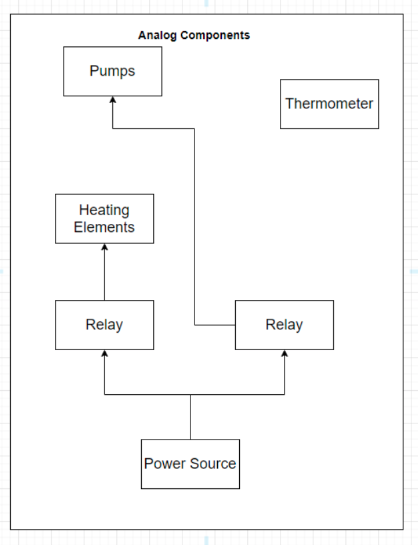
\includegraphics[width=0.60\textwidth]{images/Analog_System_Vessels.png}
	\caption{Analog System Vessel Layer Representation}
\end{figure}



\subsection{Heating Elements Subsystem}
This subsystem is used for temperature control of Hot liquor tank and the Boiling Kettle. Specifically the subsystem contains the heating elements and the Relay responsible for managing temperature control.



\subsubsection{Subsystem Hardware}
This subsystem will have heating elements, and a control relay.

\subsubsection{Subsystem Operating System}
This subsystem will have no operating system.

\subsubsection{Subsystem Software Dependencies}
There is no software dependencies.

\subsubsection{Subsystem Programming Languages}
There is none all programming and control will be done by the digital components layer.

\subsubsection{Subsystem Data Structures}
This will be the case for relay control we should be using as simple of a Data structure as possible because anything more is unnecessary because the relay just need a on or off signal. 

\subsubsection{Subsystem Data Processing}
For relay power control we should do a decent amount of testing to judge the delay that we are operating on for temperature management.



\subsection{Pump Control Subsystem}
This subsystem will be used for flow control of the entire system.



\subsubsection{Subsystem Hardware}
This subsystem will contain the pumps, and a control relay.

\subsubsection{Subsystem Operating System}
This subsystem will have no operating system.

\subsubsection{Subsystem Software Dependencies}
There is no software dependencies.

\subsubsection{Subsystem Programming Languages}
There is none all programming and control will be done by the digital components layer.

\subsubsection{Subsystem Data Structures}
This will be the case for relay control we should be using as simple of a Data structure as possible because anything more is unnecessary because the relay just need a on or off signal. 

\subsubsection{Subsystem Data Processing}
For relay power control we should do a decent amount of testing to judge the delay that we are operating on for temperature management.



\subsection{Power Control Subsystem}
This subsystem will be controlling the electric current to the relays and the Heating Elements.


\subsubsection{Subsystem Hardware}
This subsystem contains all relays ,the Power source and the Heating Elements.


\subsubsection{Subsystem Operating System}
This subsystem will have no operating system.

\subsubsection{Subsystem Software Dependencies}
There is no software dependencies.

\subsubsection{Subsystem Programming Languages}
There is none all programming and control will be done by the digital components layer.

\subsubsection{Subsystem Data Structures}
The data structure will be similar to the others in testing and requirements. 

\subsubsection{Subsystem Data Processing}
For data processing we should be stuttering the on and off states of the relays to simulate a more precise control of the power flow.





\subsection{Thermometer Control Subsystem}
This subsystem will be providing the power to the thermometer


\subsubsection{Subsystem Hardware}
The subsystem contains the power supply and the Thermometer.


\subsubsection{Subsystem Operating System}
This subsystem will have no operating system.

\subsubsection{Subsystem Software Dependencies}
There is no software dependencies.

\subsubsection{Subsystem Programming Languages}
There is none all programming and control will be done by the digital components layer.

\subsubsection{Subsystem Data Structures}
None you will simply be providing power

\subsubsection{Subsystem Data Processing}
None you will simply be providing power
